\title{INTD290: Number Systems in pre-Columbian Context}
\author{Dr. Jordan Hanson - Whittier College Dept. of Physics and Astronomy}
\date{\today}
\documentclass[10pt]{article}
\usepackage[a4paper, total={18cm, 27cm}]{geometry}
\usepackage{outlines}
\usepackage{hyperref}
\usepackage{graphicx}
\begin{document}
\maketitle

\section{How to Submit this Assignment}

Once you answer the questions, take a picture of your work and convert it to a PDF.  Submit the PDF to the assignment link on Moodle.

\section{Introduction to Digits and Bases}

\textbf{[Asynchronous Lesson 0.1: corresponding video]} In pre-Columbian scientific communities, we do not encounter the same systems of numbers as those used within the European scientific revolution.  Based on the video 0.1, answer the following questions.

\begin{enumerate}
\item Imagine seeing four people standing under a tree.  which of the following symbols describes the number of people under the tree?
\begin{itemize}
\item A: \textit{4}
\item B: $....$
\item C: \textit{- - - -}
\item D: \textit{all of the above}
\end{itemize}
\item How many digits are there in the hexidecimal system?
\begin{itemize}
\item A: 8
\item B: 10
\item C: 16
\item D: 20
\end{itemize}
\item Write the number 255 as the sum of digits times powers of 10, as in video 0.1. \\ \vspace{2cm}
\item How do you write 12 in hexidecimal?
\begin{itemize}
\item A: 12
\item B: C
\item C: D
\item D: 1A
\end{itemize}
\item Let's convert the number 255 to hexidecimal, a base-16 number system.  (a) First, divide 255 by 16 and start a column of the remainders.  (b) Divide the result of (a) by 16 again, and record the remainder.  (c) Repeat this process until the result is less than 16.  This is your final remainder, because you can't divide by 16 again.  (d) Line up the remainders to get the hexidecimal expression for 255. \\ \vspace{3cm}
\end{enumerate}

\section{Base-2 Systems and Base-20 Systems}

\textbf{[Asynchronous Lesson 0.2: corresponding video]}  We move forward with base-2 or binary number systems.  Watch the video 0.2 and answer the following questions.

\begin{enumerate}
\item Convert the following binary numbers to decimal numbers:
\begin{itemize}
\item 1000
\item 1001
\item 1101
\item 1111
\end{itemize}
\item Convert the following decimal numbers to binary numbers:
\begin{itemize}
\item 32
\item 42
\item 11
\item 17
\end{itemize}
\item Suppose we introduce a base-20 number system.  We need 20 digits, including 0-19.  Use the Arabic numerals 0-9, plus letters from the alphabet A-K as digits representing the numbers 10-19.  (a) What are the first three powers of 20: $20^0$, $20^1$, $20^2$? (b) So how would you represent the decimal number 400 in your base-20 system? (c) How would you represent 401? \\ \vspace{2cm}
\item Convert the following numbers to your base-20 system:
\begin{itemize}
\item 25
\item 45
\item 425
\item 625
\end{itemize}
\end{enumerate}

\section{The Mayan Number System}

\textbf{[Asynchronous Lesson 0.3: corresponding video]}  We finish the lesson with the Mayan number system.  Watch the video 0.3 and answer the following questions.

\begin{figure}[hb]
\centering
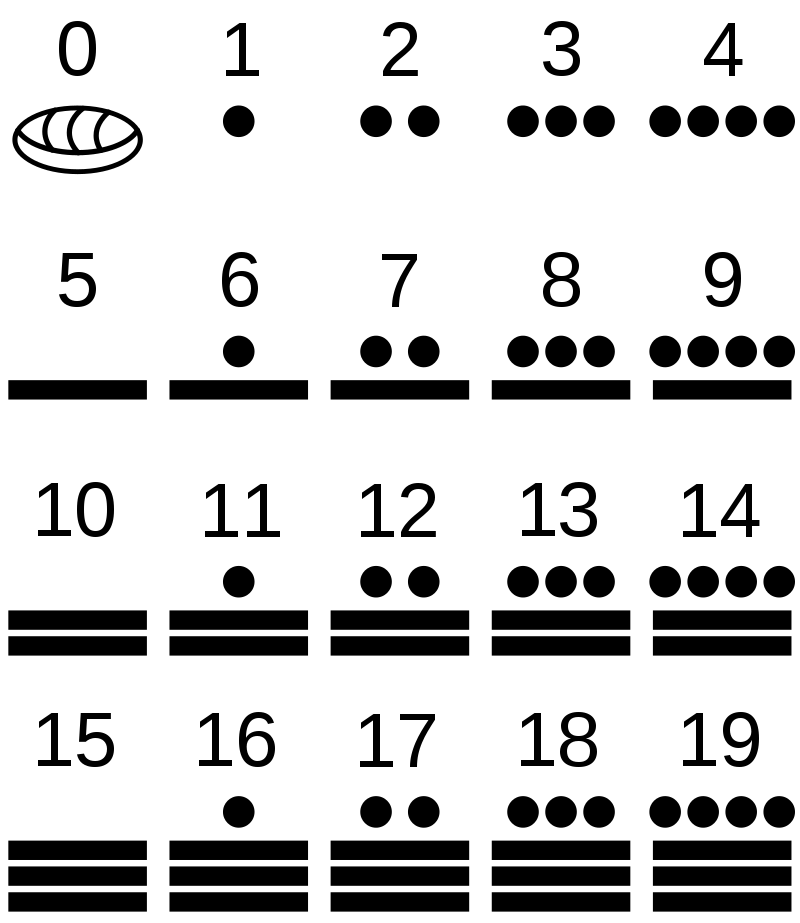
\includegraphics[width=3cm]{figures/maya_digits.png}
\caption{\label{fig:maya} The 20 digits of the Mayan system.  The digit for 0 resembles an empty shell.  The dots are worth 1 and the bars are worth 5.}
\end{figure}

\begin{enumerate}
\item You've converted the following numbers to base-20:
\begin{itemize}
\item 25
\item 45
\item 425
\item 625
\end{itemize}
Now write these numbers as the Mayans wrote them, using the digits in Fig. \ref{fig:maya}.  Subtract 20 from each of them, and write the results using Mayan digits.  (You can put your work on a separate page).
\end{enumerate}

\end{document}
